\documentclass[a4paper,10pt]{article}
\usepackage[T1]{fontenc}
\usepackage[utf8]{inputenc}
\usepackage{epsfig}
\usepackage{amssymb,amsmath,amsthm,mathrsfs,mathtools,amscd}
\usepackage{natbib}
\usepackage{float}
\usepackage[figtopcap]{subfigure}
\usepackage{mymacros}
\usepackage{pgfplots}
% \pgfplotsset{compat=newest}
% \usetikzlibrary{external}
% \tikzexternalize[prefix=tikz/]
\usepackage[bookmarks=true]{hyperref}

% \input{mathComAbb} %uses mathcomabb.tex to define commands for symbols and notations 

\newtheorem{theorem}{Theorem}[section]
\theoremstyle{definition}
\newtheorem{definition}[theorem]{Definition}

%opening
\title{Concepts for the Lecture on MOR}
\author{Jan Heiland}



\begin{document}
\maketitle
\begin{abstract}
	This file contains only the course of the lectures that I have setup to replace or enhance parts of the short course by Peter Benner as given at Fudan University in 2013. Please see the lecture notes for the actual content of the course.
\end{abstract}
\tableofcontents
\def\abcsys{\ensuremath{(A,B,C,-)}}
\def\abcdsys{\ensuremath{(A,B,C,D)}}
\def\eabcsys{\ensuremath{(E;A,B,C,-)}}
% \def\abcsyst{\ensuremath{(TAT^{-1},TB,CT^{-1},-)}}
\def\abcdsyst{\ensuremath{(TAT^{-1},TB,CT^{-1},D)}}
\def\tfabcds{\ensuremath{C(sI-A)^{-1}B+D}}
\def\abcsyst{\ensuremath{(TAT^{-1},TB,CT^{-1},-)}}
\def\rabcdsys{\ensuremath{(\hA,\hB,\hC,\hD)}}
\providecommand{\inva}[1]{\text{~\textup{d}} #1}
\providecommand{\norm}[1]{\lVert#1 \rVert}
\providecommand{\abs}[1]{\lvert#1\rvert}

\def\sco{_{co}}
\def\sbco{_{\bar c o}}
\def\sbcbo{_{\bar c \bar o}}
\def\scbo{_{c \bar o}}

\def\Rplus{\mathbb R_{\geq 0}}
\def\htwo{\ensuremath{\mathcal H_2}}
\def\hinf{\ensuremath{\mathcal H_\infty}}
\def\edrznv{E^{\mathsf{D}}}
\def\adrznv{A^{\mathsf{D}}}


\section{Introduction to LTI Systems}
\subsection{Examples}
\begin{itemize}
	\item Heat equation observation
\end{itemize}
\subsection{State Space Systems}
\begin{align}\label{eq:lti}
	Ex(t) &= Ax(t) + Bu(t), \quad x(0) = x_0, \\
	y(t) &= Cx(t),
\end{align}
where 
\begin{itemize}
	\item $x(t) \in \Rn$: the system's state
	\item $u(t) \in \Rm$: the input or control
	\item $y(t) \in \Rq$: the output or measurements
	\item $E \in \Rnn$ is often the identity or the mass matrix of a discretization
	\item $A \in \Rnn$: the system matrix
	\item $B \in \Rnm$: the input matrix
	\item $C \in \Rqn$: the output matrix
\end{itemize}

We denote the LTI by $\abcsys$

Sometimes the state $x$ has a meaning in the model - like the temperature. Sometimes $x$ is not available or simply not of interest. Sometimes $x$ is just a mathematical object as a part of the model. 

\subsection{Transferfunctions}
The state is not accessible, not of interest or only an artificial object of the model for the input to output behavior $\mathbf G$ of a system $\mathbf P$
\begin{figure}[h]
\centering
\begin{tikzpicture}
 \draw [->] (3,1.1/2) -- (4,1.1/2); 
 \draw (4,0) rectangle (6,1.1) node[pos=.5] {$\mathbf P$};
 % \draw (4,0) rectangle (6,1.1) node[pos=.5] {\small{$y(t) = Cx(t), Ex(t) = Ax(t) + Bu(t)$}};
 \draw [->] (6,1.1/2) -- (7,1.1/2); 
 \node at (2.7,0.5) {$u$};
 \node at (7.3,0.5) {$y$};
\end{tikzpicture}
\end{figure}
that maps an input $u$ to the corresponding output $y$.

If $\mathbf P$ is an $\abcsys$, the function $\mathbf G$ can be defined via 
\begin{equation*}
	\mathbf P \colon u \mapsto y\colon y(t) = S(t, u)
\end{equation*}
this is time-domain. A function $u \colon [0, \infty) \to \Rm$ is mapped to a function $y\colon [0, \infty)  \to \Rq$.

Through the Laplace transform $\mathcal L$ and its inverse $\mathcal L^{-1}$, we can switch between time-domain and frequency-domain representations of the input and output signals.

\begin{equation*}
	U(s) := \mathcal L\{u\}(s) := \int_0^\infty e^{-st}u(t)\inva t,
\end{equation*}
where $s\in \mathbb C$ is the \emph{frequency} and
\begin{equation*}
	y(t) := \mathcal L^{-1}\{Y\}(t) := \lim_{T\to \infty} \frac 1{2\pi i} \int_{\gamma - iT}^{\gamma + iT} e^{s}Y(s)\inva s
\end{equation*}
where $\gamma \in \R$ is chosen such that contour path of the integration is the domain of convergence of $Y$.

With the basic properties of the Laplace transform
\begin{itemize}
	\item $\dot X(s):= \mathcal L\{\dot x\}(s) -x(0)= s\mathcal L\{x\}(s) = s X(s)-x(0)$
	\item and linearity $\mathcal L\{Ax\}(s) = AX(s)$
\end{itemize}
with zero initial value $x(0) = 0$, the $\abcsys$ defines the transferfunction
\begin{equation*}
	G(s) := C(sE-A)^{-1}B
\end{equation*}

\subsection{Realizations}
Given a rational matrix function $s\mapsto G(s)\in \mathbb R^{q\times m}$, is there $\abcsys$ so that 
\begin{equation*}
	G(s) = C(sI-A)^{-1}B ?
\end{equation*}
If there is one such state space system $\abcsys$, then there are infinitely many:

For every invertible $T$, the state space system $\abcsyst$ is a realization, since
\begin{equation*}
	C(sI-A)^{-1}B = CT^{-1}(s-TAT^{-1})^{-1}TB.
\end{equation*}

Also
\begin{equation*}
	(
	\begin{bmatrix} A & 0 \\ 0 & 0 \end{bmatrix},
	\begin{bmatrix} B \\ 0 \end{bmatrix},
	\begin{bmatrix} C & 0 \end{bmatrix}, -
	)
\end{equation*}
is a realization of one and the same transferfunction.

Thus, there are many possible state space representations of a transfer function. Which one is a good choice? The dimension can be arbitrary large. How small can it be? (cf. \emph{model reduction})

\subsection{Controllability, Observability}

The states of an LTI are just part of a model that realizes a transfer function $G$. A transferfunction $G$ describes how controls $u$ lead to outputs $y$. As seen above in the example, there can be states that are neither affected (\emph{controlled} by the inputs nor seen (\emph{observed}) by the outputs of the system and which are obviously not needed to realize the input to output behavior of $G$.  

We will give a thorough characterization of the \emph{controllable} and \emph{observable} states of an LTI. 

\begin{definition}
	The LTI $\abcsys$ or the pair $(A, B)$ is said to be \emph{controllable} if, for any initial state $x(0) = x_0$, $t_1 > 0$ and final state $x_1$, there exists a (piecewise continuous) input $u$ such that the solution of \eqref{eq:lti} satisfies $x(t_1 ) = x_1$. Otherwise, the system $\abcsys$ or the pair $(A, B)$ is said to be \emph{uncontrollable}.
\end{definition}


\begin{definition}
	The LTI \abcsys~ or the pair $(C,A)$ is said to be \emph{observable} if, for any $t_1 > 0$, the initial state $x(0) = x_0$ can be determined from the time history of the input $u$ and the output $y$ in the interval of $[0, t_1]$. Otherwise, the system \abcsys, or $(C, A)$, is said to be \emph{unobservable}.
\end{definition}

There are algebraic conditions on controllability and observability.

\begin{theorem}
	The LTI $\abcsys$ is controllable (observable) if, and only if, the transformed LTI $\abcsyst$ is controllable (observable), where $T$ is a regular matrix.
\end{theorem}

With these definitions, and the invariance of the properties and the transferfunction with respect to state space transformations, we can find the states that really matter for the realization of a transferfunction.

\begin{theorem}[Kalman Canonical Decomposition]
	Given an LTI $\abcsys$, there is a state space transformation $T$ such that the transformed system $\abcsyst$ has the form 

	\begin{align*}
		\frac {\inva{}}{\inva t}
		\begin{bmatrix} x_{co} \\ x_{c\bar o} \\ x_{\bar c o} \\ x_{\bar c \bar o} \end{bmatrix} 
			&= 
		\begin{bmatrix}
			A\sco & 0 & A_{13} & 0 \\
			A_{21} & A\scbo & A_{23} & A_{24} \\
			0 & 0 & A\sbco & 0 \\
			0 & 0 & A_{43} & A\sbcbo 
		\end{bmatrix}
		\begin{bmatrix} x_{co} \\ x_{c\bar o} \\ x_{\bar c o} \\ x_{\bar c \bar o} \end{bmatrix}
			+
		\begin{bmatrix} B\sco \\ B\scbo \\ 0 \\ 0 \end{bmatrix} u \\
			y &= 
			\begin{bmatrix} C\sco & 0 & C\sbco & 0 \end{bmatrix}
		\begin{bmatrix} x_{co} \\ x_{c\bar o} \\ x_{\bar c o} \\ x_{\bar c \bar o} \end{bmatrix},
	\end{align*}
	with the subsystem $(A\sco, B\sco, C\sco, -)$ being controllable and observable, while the remaining states $x\sbco$, $x\scbo$, or $x\sbcbo$ are not controllable, not observable, or neither of them.
	Moreover, for the transferfunction, it holds that
	\begin{equation*}
		G(s) = C(sI-A)^{-1}B = C\sco(sI-A\sco)^{-1}B\sco.
	\end{equation*}
\end{theorem}

What does this mean for us and a transferfunction $G(s)$?
\begin{itemize}
	\item The minimal dimension of a realization is the dimension of $x\sco$ in the \emph{Kalman Canonical Decomposition}
	\item Such a realization is called \emph{minimal realization}
	\item It is the starting point for further model reduction. (Throwing out $x\sbco$ etc. does not effect $G(s)$ and is typically not considered a model reduction)
	\item There are algorithm to reduce a realization to a minimal one (cf. Varga)
	\item In practice, the uncontrolled and unobserved states play a role and they may cause troubles ( check the literature for \emph{zero dynamics} )
\end{itemize}

\subsection{Stability}
A system $G$ is stable if all \emph{poles} of $G$ are located in the left half-plane $\C^-$.

{\footnotesize If $m=q=1$, then $G(s)=\frac{N(s)}{D(s)}$, where $N(s)$ and $D(s)$ are polynomials and the \emph{poles} are the roots of $D(s)$, i.e. those $s\in\mathbb C$ for which $D(s)=0$.

If $m$, $q >1$, then one can use the \emph{McMillan} form of $G$ to determine the poles.}

If \abcdsys~is a minimal realization of a stable system $G$, then the poles of $G$ are the eigenvalues of $A$.

In this case, the system is stable if for all eigenvalues $\lambda$ of $A$, it holds that $\lambda \in \C^-$. Then $A$ is called \emph{stable} or \emph{Hurwitz}.

A stable system can have a stable realization.


\subsection{Gramians and Balanced Realizations}
If $A$ is stable, then the \emph{Lyapunov} equations 
\begin{align*}
	A^*P + PA + BB^* = 0
	\intertext{and}
	AQ + Q^*A + C^*C = 0
\end{align*}
have a unique positive definite solutions $P$ and $Q$. The matrix $P$ is called the the controllability Gramian and $Q$ is called the observability Gramian.

If $P$ and $Q$ are the Gramians of a stable realization \abcdsys, then the transformed system $\rabcdsys=\abcdsyst$ has the Gramians 
\begin{equation*}
	\hat P = TPT^* \quad \text{and} \quad \hQ = (T^{-1})^*QT^{-1}
\end{equation*}
for any regular transformation $T$.

For any minimal and stable system $\abcdsys$, there are particular transformations $T$, so that the transformed system has Gramians that are equal and diagonal:
\begin{equation*}
	\hat P = \hQ =
	\begin{bmatrix}
		\lambda_1 & & & \\
		& \lambda_2 & & \\
		& & \ddots & \\
		& & & \lambda_n \\
	\end{bmatrix},
\end{equation*}
with $\lambda_1 \geq \lambda_2 \geq \dotsm \geq \lambda_n > 0$.

These realizations are called \emph{Balanced Realizations}.


% \section{Norms of Signals and Systems}
\subsection{Norms}

Ingredients of a norm:
\begin{itemize}
	\item A linear space $V$ over $\mathbb C$ (or $\mathbb R$).
	\item A functional $$\norm{\cdot}\colon V \to \Rplus$$ that has the following properties:
		\begin{enumerate}
			\item $\norm{\alpha v} = \abs{\alpha}\norm{v}$,
			\item $\norm{v+w} \leq \norm{v}+\norm{w}$, and
			\item $\norm{v} = 0$ if, and only if, $v=0$,
		\end{enumerate}
		for any $v$, $w\in V$ and any $\alpha \in \mathbb C$ (or $\mathbb R$).
\end{itemize}

If $(V,\norm{\cdot}_V)$ and $(W,\norm{\cdot}_W)$, then for the space of linear maps $\bigl ( V \to W \bigr)$ a norm is defined via
$$
\norm{G}_* := \sup_{v\in V, v\neq 0}\frac{\norm{Gv}_W}{\norm{v}_V}.
$$
This is the norm for $G\colon V \to W$ that is induced by $\norm{\cdot}_V$ and $\norm{\cdot}_W$. There can be other norms that are not induced.

\subsection{Norms of Signals}
Common norms and spaces for the input and output signals 
$$u, y\colon [0, \infty) \to \mathbb R^{m}, \mathbb R^{q}$$:

The $\bL_1^m$ norm 
$$ \norm{u}_{\bL_1} := \int_0^\infty \sum_{i=1}^m\abs{u_i(t)} \inva t $$ 
that defines the $\bL_1^m$ space of integrable (summable) functions
$$\bL_1^m:=\bigl \{ u \colon [0, \infty) \to \mathbb R^{m} : \norm{u}_{\bL_1}<\infty \bigr \} $$

The $\bL_2^q$ norm 
$$ \norm{y}_{\bL_2} := \bigl(\int_0^\infty \sum_{i=1}^q\abs{y_i(t)}^2 \inva t\bigr)^{\frac 12} $$ 
that defines the $\bL_2^q$ space of square integrable functions
$$\bL_2^q:=\bigl \{ y \colon [0, \infty) \to \mathbb R^{q} : \norm{u}_{\bL_1}<\infty \bigr \} $$

The $\bL_\infty^m$ norm 
$$ \norm{u}_{\bL_\infty} := \max_{i=\{1, \dotsc, m\}} \sup_{t>0}\abs{u_i(t)} $$ 
that defines the $\bL_\infty^m$ space of bounded functions
$$\bL_\infty^m:=\bigl \{ u \colon [0, \infty) \to \mathbb R^{m} : \norm{u}_{\bL_\infty}<\infty \bigr \} $$

Where it is clear from the context, we will drop the superscripts $p$ and $m$ that denote the dimension of the signals.

The $\bL_2 $ norm can also be evaluated in frequency domain

\begin{theorem}
	For $u \in \bL_2 $ it holds that 
	\begin{equation*}
		\norm{u}_{\bL_2 } = \bigl ( \frac{1}{2\pi} \int_{-\infty}^{\infty} U(i\omega)^*U(i\omega) \inva \omega \bigr)^{\frac 12},
	\end{equation*}
	where $U$ is the \emph{Fourier} transform of $u$.
\end{theorem}

\begin{footnotesize}
	Fourier transform $\mathcal F$ and Laplace transform $\mathcal L$ coincide for $s=i\omega$, $\omega \in \mathbb R^{}$ and  $u(t)=0$ for $t\leq 0$:
	$$
	\mathcal F(u)(i\omega) := \int_{-\infty}^{\infty} u(t) e^{-i\omega t}\inva t = \int_0^{\infty} u(t)e^{-st}\inva t = \mathcal L(u)(s)
	$$
\end{footnotesize}
\subsection{Norm of a System}
A system $G$ or \abcdsys transfers inputs to outputs.
\begin{itemize}
	\item What does a norm mean for a system?
	\item Or, what is a large system, what is a small system?
\end{itemize}
From the definition of an operator norm.

$$
\norm{G} = \sup_{u\neq 0}\frac{\norm{Gu}}{\norm{u}} 
$$
meaning that for all $u$:
$$
\norm{y}=\norm{Gu}\leq \norm{G}\norm{u}.
$$

For systems, large refers to what extend an input is amplified and $\norm{G}$ is called the \emph{gain}.

Furthermore, with a norm one can compare two systems $G_1$ and $G_2$ via the difference in the output for the same input

$$\norm{y_1 - y_2 }=\norm{G_1u - G_2u}\leq \norm{G_1-G_2}\norm{u}.$$

\subsection{Defining a norm for systems}
Let $m=q=1$, i.e. we consider a SISO system \abcsys.

If \abcsys with stable and strictly proper transfer function $G$ is stable, then impulse response of the system
$$g(t) = C\int_0^t e^{A(t-s)}B\delta(s) \inva s = Ce^{At}B$$
decays exponentially and 
$$
\norm{g}_{\bL_2 } = \bigl( \frac{1}{2\pi} \int_{-\infty}^{\infty} G(i\omega)^*G(i\omega) \inva \omega \bigr)^{\frac 12} =: \norm{G}_2 < \infty
$$
This defines a norm for systems since (Exercise!)
\begin{itemize}
	\item $G=C(sI-A)^{-1}B$ is indeed the Laplace transform of $g$
	\item the functional $\norm{\cdot}_2$ for stable and strictly proper transferfunctions is a norm
\end{itemize}

Furthermore, (Exercise!), $\norm{y}_{\bL_\infty} \leq \norm{G}_2 \norm{u}_{\bL_\infty}$.

\begin{footnotesize}
	A system \abcdsys~or $A$ is stable, if there exists a $\lambda>0$, such that $\norm{e^At}\leq e^{-\lambda t}$, for $t>0$. This means that all eigenvalues of $A$ must have a negative real part.
\end{footnotesize}


For MIMO systems \abcsys~with $u(t)\in\Rm$ and $y(t)\in\Rq$, with a stable and strictly proper transferfunction $\mathcal G\colon s \to \mathbb R^{q\times m} $, the $\htwo$ norm is defined as  
\begin{equation*}
	\norm{G}_2 := \bigl( \frac{1}{2\pi} \int_{-\infty}^{\infty} \trace{ G(i\omega)^*G(i\omega)} \inva \omega \bigr)^{\frac 12}
\end{equation*}

This is the norm of the well-known $\emph{Hardy}$ space $\htwo$ of matrix functions that are analytic in the open right half of the complex plane. Stable and strictly proper transfer functions are in $\htwo$.

For a stable and proper transfer function one can define the $\hinf$ norm:
\begin{equation*}
	\norm{G}_\infty := \sup_{\omega \in \mathbb R^{} } \sigma_{\max{}} \bigl(G(i\omega)\bigr),
\end{equation*}
where $\sigma_{\max{}}\bigl(G(i\omega)\bigr)$ is the largest singular value of $G(i\omega)$.

This is the norm of the well-known $\emph{Hardy}$ space $\hinf$ of matrix functions that are analytic in the open right half of the complex plane and bounded on the imaginary axis. Stable and strictly proper transfer functions are in $\htwo$.

The $\hinf$-norm is induced by the $\bL_2$ norm:
\begin{equation*}
	\norm{G}_\infty = \sup_{u\in \bL_2, u\neq 0}\frac{\norm{Gu}_{\bL_2}}{\norm{u}_{\bL_2}} .
\end{equation*}

\section{Linear Time-invariant DAEs}

\subsection{System Theoretic Aspects of DAEs}
Consider
\begin{align*}
	Ex(t) &= Ax(t) + Bu(t), \quad x(0) = x_0, \\
	y(t) &= Cx(t),
\end{align*}
where
\begin{itemize}
	\item $x(t) \in \Rn$: the system's state
	\item $u(t) \in \Rm$: the input or control
	\item $y(t) \in \Rq$: the output or measurements
	\item $E \in \Rnn$ is \emph{singular}
	\item $A \in \Rnn$: the system matrix
	\item $B \in \Rnm$: the input matrix
	\item $C \in \Rqn$: the output matrix
\end{itemize}
we will denote the system by \eabcsys.

Often, these \eabcsys~are referred to as \emph{descriptor} or \emph{singular} systems.

The transfer function of an \eabcsys~in time domain is given as
	\begin{align*}
		&\mathbf G \colon u \mapsto y\colon\\
		&\quad y(t) = C \bigl[e^{\edrznv At}x_0 + \int_0^te^{\edrznv A(t-s)}\edrznv Bu(s)\inva s \bigr] - (I-\edrznv E) \sum_{i=0}^{\nu-1}(E\adrznv )^i\adrznv Bu^{(i)}(t)\bigr] ,
	\end{align*}
	where
	\begin{itemize}
		\item $\edrznv$ is the \emph{Drazin} inverse of $E$
		\item $\nu$ is the \emph{differentiation index} of the DAE $E\dot x = Ax$
		\item $u^{(i)}$ denotes the $i$-th derivative of $u$
	\end{itemize}

	Note that if $E=I$, then $\edrznv = I$ and the transfer function is given as
	\begin{equation*}
		\mathbf G \colon u \mapsto y\colon y(t) = C \bigl[e^{At}x_0 + \int_0^te^{A(t-s)}Bu(s)\inva s \bigr]+ Du(t),
	\end{equation*}
	known as the formula of \emph{variation of constants}.


	In frequency domain (after a \emph{Laplace} transform) the transfer function is given as
	$$G(s) = C(sE-A)^{-1}B$$
	but, depending on $B$ and $C$ it can be \emph{improper}. That is, possibly,
	$$\norm{G(s)} \to \infty \quad\text{as }s\to \infty$$
	Since standard model reduction approaches return a \emph{proper} reduced system $\hat G$, this will happen (cf. \cite{morGugSW13})

		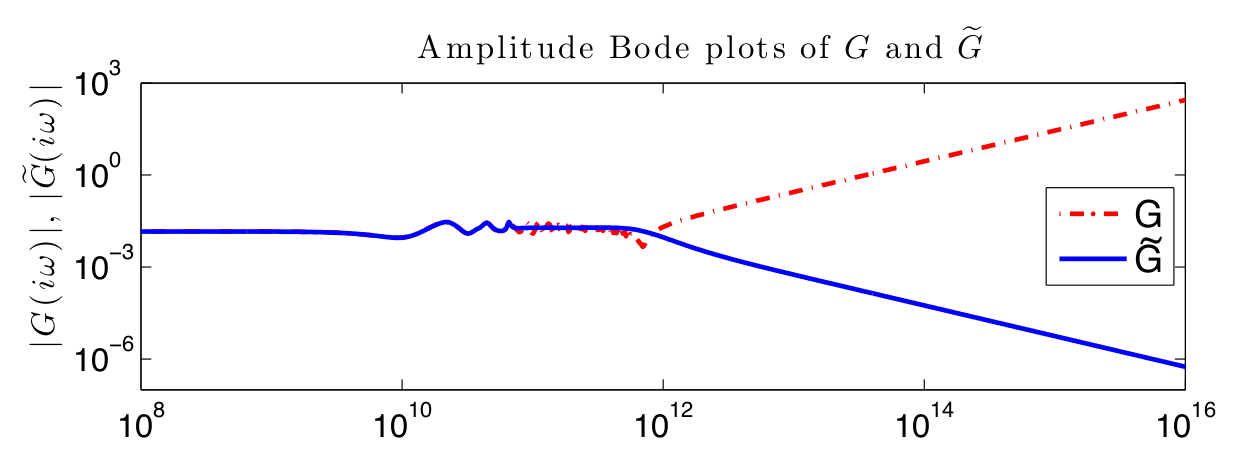
\includegraphics[width=\textwidth]{GugSW-properimproper}

	The general problem is:
	\begin{itemize}
		\item the transfer function can have an improper part (frequency domain)
		\item the system differentiates the input (time domain)
	\end{itemize}

	The general approach is:
	\begin{enumerate}
		\item Project the DAE onto the part that is an ODE, i.e. a standard state space system
		\item Keep the remainder, i.e. the algebraic or improper part, as it is 
	\end{enumerate}
	This means: \emph{no model reduction on the algebraic part!}

\subsection{Balanced Truncation for Navier-Stokes Systems}
  We consider linearized Navier-Stokes equations:
	\begin{align*}
		M \dot v(t) &=  A_1v(t) + J^T p(t) + B_1 u(t), \\
		Jv(t) &= 0, \\
		y(t) &= C_1v(t).
	\end{align*}

\begin{itemize}
	\item $v(t) \in \Rn$: one system's state (velocity)
	\item $p(t) \in \Rp$: another system's state (pressure)
	\item $u(t) \in \Rm$: the input or control
	\item $y(t) \in \Rq$: the output or measurements
	\item $M \in \Rnn$ is the mass matrix (non singular)
	\item $A_1 \in \Rnn$: the system matrix
	\item $B_1 \in \Rnm$: the input matrix
	\item $C_1 \in \Rqn$: the output matrix
\end{itemize}

Note that this is an \eabcsys~with
\begin{equation*}
	E:= \begin{bmatrix} M & 0 \\ 0 & 0 \end{bmatrix}, \quad
	A:= \begin{bmatrix} A_1 & -J \\ J^T & 0 \end{bmatrix}, \quad
	B:= \begin{bmatrix} B_1 \\ 0\end{bmatrix}, \quad \text{and}\quad
	C:= \begin{bmatrix} C_1 & 0 \end{bmatrix}.
\end{equation*}

Simplifying properties and assumptions:
\begin{itemize}
	\item linearity -- the Navier-Stokes equations are nonlinear
	\item stability -- this is only true for slowly moving flows
	\item ``$B_2=0$'' and ``$C_2=0$'': the improper part is zero
\end{itemize}




\bibliographystyle{plain}
\bibliography{mor}
\end{document}

